
\documentclass[]{article}

\usepackage{amsmath}
\usepackage{graphicx}

%opening
\title{Zeitreisen}
\author{Jonas Gr\"undler, Sascha Jecklin}

\begin{document}

\maketitle



\section{Einleitung}
	 Das Thema Zeitreisen fasziniert den Menschen schon seit langem. Bereits in der Hinduistischen Mythologie und in der Budhistischen Religion besch\"aftige man sich mit Reisen in der Zeit. Auch in der modernen Literatur und in der Science-fiction sind Zeitreisen ein verbreitetes Thema. Klassische Beispiele daf\"ur w\"aren: 
	 
	 \begin{itemize}
	 	\item Time Machine, H.G.Wells, 1895 
	 	\item Das Ende der Ewigkeit, Isaac Asimov, 1955
	 	\item Back to the Future, 1985-1990
	 	\item Star Trek
	 	\item Doctor Who
	 	\item \ldots
	 \end{itemize}
 
	 Doch was sind Zeitreisen genau und sind Sie \"uberhaupt m\"oglich? Diese Frage versuchen Wir hier im Rahmen dieser Arbeit zu beantworten.
	 Grunds\"atzlich gibt zwei Arten von Zeitreisen:
	
	\begin{itemize}
		\item In die Zukunft
		\item In die Vergangenheit
	\end{itemize}
	
	Wir werden uns in dieser Arbeit auf Zeitreisen in die Zukunft beschr\"anken. Nach aktuellem Stand der Wissenschaft sind Zeitreisen in die Vergangenheit nicht m\"oglich. Es existieren Theorien doch diese sind umstritten und spekulativ.
	
\section{Was ist eine Zeitreise}
	Was versteht man unter einer Zeitreise? Es bezeichnet eine Bewegung in der Zeit, die vom gew\"ohnlichen Zeitablauf abweicht. In der Physik kann dieser Effekt durch die Zeitdilatation erreicht werden. Also, wenn die Zeit f\"ur einem Langsamer vergeht als f\"ur ein Bezugssystem. Dies kann durch verschiedene Arten erreicht werden. Wir beschr\"anken uns hier auf zwei Arten:
	
	\begin{itemize}
		\item Geschwindigkeit
		\item Gravitation	
	\end{itemize}

	In den n\"achsten zwei Unterkapiteln untersuchen wir je einen dieser Faktoren
	
\subsection{Geschwindigkeit}

	Eine M\"oglichkeit diesen eine Zeitdillatation zu erreichen ist durch hohe Geschwindigkeit. Wenn sich eine Person relativ zu einem Bezugssystem schnell bewegt, vergeht f\"ur diese Person die Zeit im Vergleich zum Bezugssystem langsamer. Die Ver\"anderung wird durch den Lorentzfaktor beschrieben, welcher sich aus der Lorentztransformation herleiten l\"asst. Er beschreibt das Verh\"altnis zwischen der Eigenzeit und der Zeit des Bezugssystems.
	
	\begin{equation}
	 	\gamma=\frac{1}{\sqrt{1-\frac{v^2}{c^2}}} 
	\end{equation}
	
	
	
	Die Eigenzeit ist also:
	
	\begin{equation}
		\tau
		=
		\int_{}^{}\frac{1}{\gamma}dt=\int_{}^{}\sqrt{1-\frac{v^2}{c^2}}dt
		=
		\frac{1}{c}\int_{}^{}\sqrt{g_{\mu\nu}\dot{x}^{\mu}(s)\dot{x}^{\nu}(s)}ds
	\end{equation}
	
	Diese Formel ist in dieser Form noch nicht sehr Anschaulich. Sie Beschreibt nur, dass eine Metrik mit den jeweiligen Basisvektoren "multipliziert" werden muss(Einsteinsche Summenkonvention). Von dem Ganzen die Wurzel ziehen und dann noch integrieren.
	Durch das Einsetzen der Minkowski-Metrik, welche Raum und Zeit miteinander verbindet, und der Basisvektoren $t, x, y, z$ l\"asst sich eine Verst\"andliche Form herleiten. 
	
	 Minowski-Metrik:
	 
	\begin{equation}
		g_{\mu\nu}=
   		 \begin{pmatrix}
		 		-1 & 0 & 0 & 0 \\
	    		0 & 1 & 0 & 0 \\
	 			0 & 0 & 1 & 0 \\
	  			0 & 0 & 0 & 1
	 	\end{pmatrix}
	\end{equation}
	
	Standard Vierervektor:
	 
	\begin{list}{}{}
		\item \(x^{0}=ct\)
		\item \(x^{1}=x\)
		\item \(x^{2}=y\)
		\item \(x^{3}=z\)
	\end{list}

	 Ein wenig Umstellen und vereinfachen und man kommt auf diese Form:
	 
	 \begin{equation}
	 	\tau
	 	=
	 	\frac{1}{c}\int_{}^{}\sqrt{-(-c^2\dot{t}(s)^{2}+\dot{x}(s)^{2}+\dot{y}(s)^{2}+\dot{z}(s)^{2})}ds
	 \end{equation}
	 
	 Je nachdem wie die Bewegung gew\"ahlt wird, fallen einer oder mehrere der Basisvektoren  $x, y, z$ weg.\\\\\\\\ Hier ein Beispiel bei welchem nur eine Geschwindigkeit in x-Richtung vorhanden ist(c=Lichtgeschwindigkeit, u beschreibt den Bruchteil):
	 
	 \begin{list}{}{}
	 	\item $t(s)=1s, \dot{t}(s)=1$
	 	\item $x(s)=u*c*s, \dot{x}(s)=u*c$
	 	\item $y(s)=0, \dot{y}(s)=0$
	 	\item $z(s)=0, \dot{z}(s)=0$
	 \end{list}
	 
	 \begin{align*}
	 	\tau
	 	&=
	 	\frac{1}{c}\int_{}^{}\sqrt{-(-c^2\dot{t}(s)^2+\dot{x}(s)^2)}ds 
	 	=
	 	\frac{1}{c}\int_{}^{}\sqrt{-(-c^2*1+(u*c)^{2}}ds\\
	 	&=
	 	\frac{s*\sqrt{c^2+(u*c)^{2}}}{c} 
	 	=
	 	s*\sqrt{1-\frac{u^2*c^2}{c^2}}
	 \end{align*}
	 
	 Welches die einfachste Form einer Zeitdilatation darstellt.\\
	 \\
	 Hier ein Zahlenbeispiel bei welchem zuf\"allige Werte gew\"ahlt wurden:
	 $s=5000, u=0.2$ 
	 
	 \begin{list}{}{}
	 	\item $t(s)=1s, \dot{t}(s)=1$
	 	\item $x(s)=0.2cs, \dot{x}(s)=0.2c$
		\item $y(s)=0, \dot{y}(s)=0$
		\item $z(s)=0, \dot{z}(s)=0$
	 \end{list}
	 
	 \begin{align*}
	 	\tau
	 	&=
	 	\frac{1}{c}\int_{s_{a}}^{s_{b}}\sqrt{-(-c^2\dot{t}(s)^2+\dot{x}(s)^2)}ds
	 	&=
	 	\frac{1}{c}\int_{0}^{5000}\sqrt{-(-c^2+((0.2c)^2))}ds\\
	 	&=
	 	5000*\sqrt{1-\frac{u^2*c^2}{c^2}} = 4898.98
	 \end{align*}
	 
	 Dieses Beispiel zeigt auch, dass eine relevante Zeitverlangsamung erst bei sehr hohen Geschwindigkeiten erreicht wird
	 
	 \begin{figure}
	 	\centering
	 	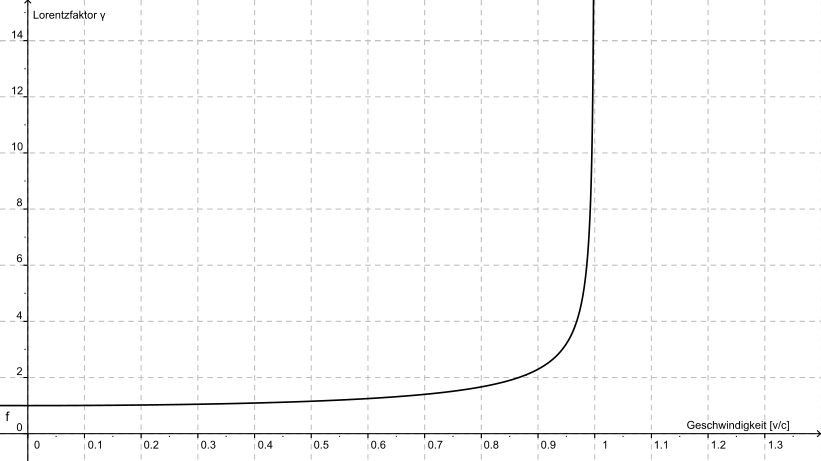
\includegraphics[width=\hsize]{Lorentzfaktor.jpg}
	 	\caption{Ver\"anderung des Lorentzfaktor in Abh\"angigkeit der Geschwindigkeit%
	 		\label{skript:geodaten:fig:transport}}
	 	\end{figure}
	 
\subsection{Gravitation}
	
	In diesem Kapitel beschäftigen wir uns mit dem Einfluss der Gravitation auf die Zeit. Gravitation muss durch eine Krümmung des Raumes beschrieben werden. Wir erkennen Die Gravitation hauptsächlich an der Anziehungskraft der Erde, alles wird mit einer Beschleunigung von $g=9.81\frac{m}{s^2}$ angezogen. $F=\frac{KMm}{r^2}$
	Die Beschleunigung ist also unabhängig von der Masse.
	Ein beschleunigtes Koordinatensystem kann zwar durch eine Koordinatentransformation erreicht werden, doch diese ist keine Lorentztransformation und enthält die Minkowski-metrik nicht. Der Ansatz $ -c^2dt^2 + dx^2 + dy^2 + dz^2$ genügt nicht mehr. Wir müssen also eine Metriken und Transformationen Zulassen welche von der Minkowski-Metrik abweichen. 
	


\end{document}
